\subsection{Definition}%
\label{subsec:kgraph_definition}
The \ac{kgraph} consists of center nodes, side nodes and edges. A center node's responsibility is to represent an object and its classification.\bs

Formally, a \textbf{center node}, $\gls{node}^{\mathit{center}}_\mathit{id} =\left\langle \mathit{id}, \mathit{id_{obj}}, \gls{objectClass} \right\rangle $\bs

Where \textit{id} an identifier for the center node, $\mathit{id_{obj}}$ an identifier for the object\\\gls{objectClass} the classification of that object which can be either MOVABLE or UNMOVABLE.\bs

\noindent A side node is a placeholder for the edge to point toward.\bs

Formally, a \textbf{side node}, $\gls{node}^{\mathit{side}}_\mathit{id} =\left\langle \mathit{id} \right\rangle $, Where \textit{id} an identifier for the side node.\bs

\noindent An edge points from center- to side node and has two responsibilities. First, it stores the parameterization used to manipulate an object that resides in the center node. Second, it stores the performance of that parameterization which is summarized in the success factor.\bs

Formally an \textbf{edge}, $\gls{edge}_{(from, to)} = \left\langle \mathit{id}_{from}, \mathit{id}_{to}, \gls{successfactor}(a), \textrm{System Model}, \textrm{Controller}\right\rangle$\bs

Where $\mathit{id}_\mathit{from}$ and $\mathit{id}_\mathit{to}$ corresond the the identifiers of the center- and side node respectively, $\gls{successfactor}(a)$ is the success factor that summarized the feedback of $a\geq0$ reviewed action edges and (System Model, Controller) together is referred to as edge parameterization. \bs

The successfactor rates an edge parameterization based on experience in the robot environment. The successfactor is created or updated when an action edge with that parameterization failed during execution time or successfully completed.\bs

Formally the \textbf{success factor} = \gls{successfactor}:
\[\gls{successfactor}(a+1) =
  \begin{cases} 0.1^{\gls{pe}_\textrm{avg}}& \textrm{if $a$ = 0}\\[5px]
    0.1 + 0.9\gls{successfactor}(a) & \textrm{if $a > 0$ and the reviewed edge was successfully completed}\\[5px]
  0.9\gls{successfactor}(a) & \textrm{if $a > 0$ and the reviewed edge failed during execution time}
\end{cases}\]

Where $\gls{pe}_\textrm{avg}$ is the average \ac{PE} of the action edge that is reviewed. $a$ is the number of times an action edge with such a edge parameterization reached the EXECUTING status.\bs

\noindent Now that the nodes and edges have been defined, the \ac{kgraph} can be defined.\bs

Formally, a \textbf{\acl{kgraph}}, $\gls{kgraph} = \left\langle \gls{nodesK}, \gls{edgesK} \right\rangle $
\\comprising $\gls{nodesK} = \{\gls{node}^{\mathit{center}}, \gls{node}^{\mathit{side}}\}$, \quad $\gls{edgesK} \in \{\gls{edge}_{(i,j)}| i \in \gls{nodesK}^\mathit{center}_\mathit{ids}, j \in \gls{nodesK}^\mathit{side}_\mathit{ids} \}$.\bs

Where $\gls{nodesK}^\mathit{center}_\mathit{ids}$ are the identifiers of the set of center nodes, and $\gls{nodesK}^\mathit{side}_\mathit{ids}$ are the identifiers of the set of side nodes.\bs

\subsection{The Testing and Converging Phases}
When the \ac{halgorithm} determines is must manipulate an object to fullfill the given task, it creates a action edge with a random edge parameterization. After executing that action edge that parameterization is stored in the \ac{kgraph}. When encountering the need to manipulate the object again a different random parameterization is selected. First, all possible edge parameterizations are tested and stored on a specific object, this can be seen as the testing phase on how to manipulate an object. Then second, when all possible parameterizations are tested, the \ac{kgraph} suggests the edge parameterization with the highest success factor, this phase can be seen as the converging phase. Where either, the edge parameterization with the highest success factor receives an even higher success factor, or the success factor is lowered, and the second best edge parameterization becomes the highest ranking edge parameterization in terms of success factor.\bs

The \ac{kgraph} has three interface functions. The \textit{add\_object(\gls{obj}, \gls{objectClass})} function adds an object and its class to the \ac{kgraph}. Espacially usefull to indicate which objects are unmovable. The \textit{add\_review(\gls{edge})} function takes an action edge from the \ac{hgraph} and depending on the \ac{kgraph} does the following. If a corresponding center node (containing the object the edge manipulated) does not yet exist, create a new center node. Then calculate the success factor and add a new edge or update the success factor of the existing edge with equal edge parameterization in the \ac{kgraph}.  

or update the the edge that containts the edge parameterization. If the edge parameterization exist in one of the outgoing edges from the center node, existthe of the corersponding object if it does not exist. 
creates or updates the corresponding edge  the \ac{kgraph} is updated with a new success factor as described in the formula above. The \textit{action\_suggestion} returns the best parameterization it contains for an object.\bs

\subsection{Legend and Example}
A legend for the \ac{kgraph} is now presented.\bs

\begin{figure}[H]
    \centering
    \begin{subfigure}{0.3\textwidth}
    \centering
    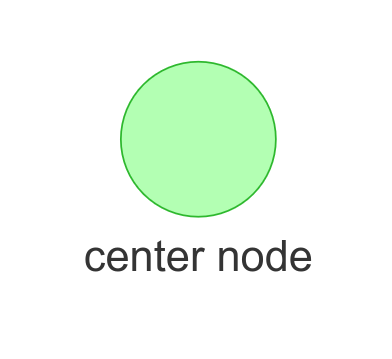
\includegraphics[width=0.9\textwidth]{figures/proposed_method/center_node}
    \caption{}%
    \end{subfigure}
    \begin{subfigure}{0.3\textwidth}
    \centering
    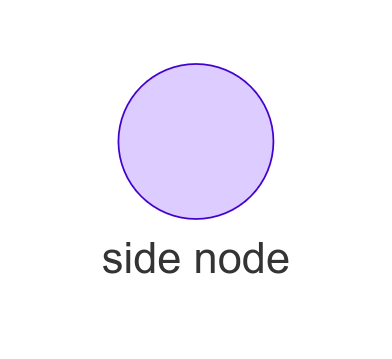
\includegraphics[width=0.9\textwidth]{figures/proposed_method/side_node}
    \caption{}%
    \end{subfigure}
    \begin{subfigure}{0.3\textwidth}
    \centering
    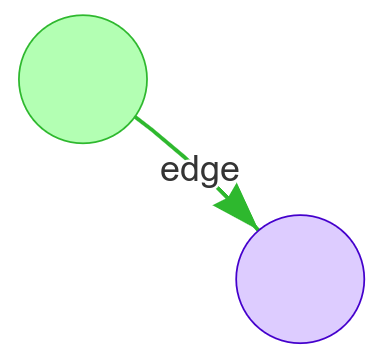
\includegraphics[width=\textwidth]{figures/proposed_method/kgraph_edge}
    \caption{}
    \end{subfigure}
    \caption{Legend for the \acl{kgraph}.}%
    \label{fig:kgraph_legend}
\end{figure}

An example \ac{kgraph} can be visualized in \Cref{fig:kgraph_example}, where edge parameterizations are displayed over the edges.\bs

\begin{figure}[H]
    \centering
    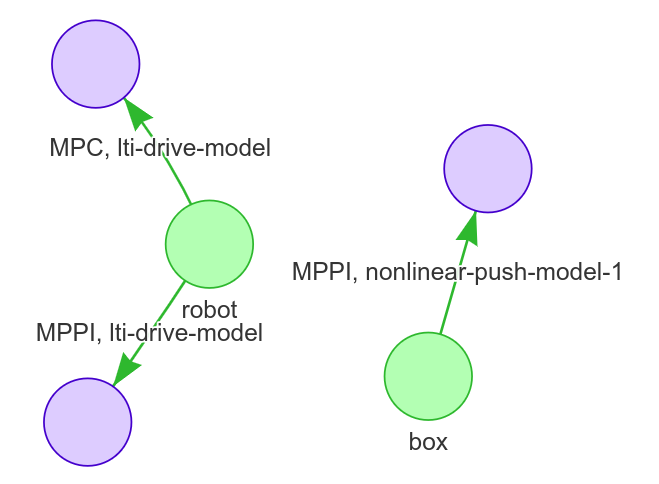
\includegraphics[width=10cm]{figures/proposed_method/kgraph_example}
    \caption{The \ac{kgraph} that has collected action feedback on two objects. Two edge parameterizations\\for driving the robot and one edge parameterization to push the box.}%
    \label{fig:kgraph_example}
\end{figure}
